\documentclass{beamer}
\usepackage[spanish]{babel}
\usepackage[utf8]{inputenc}
\usepackage{graphics}
\usepackage{amssymb} % Simbolos matematicos
\usepackage{moreverb} 
\usepackage{listings} % Para listar código

% imprimir
% \documentclass[handout]{beamer} 
% \usepackage{pgfpages}
% \pgfpagesuselayout{4 on 1}[a4paper,landscape,border shrink=5mm]

\mode<presentation> {
  \usetheme{Singapore}
%  \usetheme{Bergen}
  \useoutertheme{infolines}
  %\useoutertheme[]{miniframes}
  \usefonttheme{structurebold}
  \setbeamercovered{transparent}
}

\setbeamertemplate{headline}
{%
  
\includegraphics[height=1.5cm]{format/eoi-header.jpg}%
}

\setbeamercolor{titlelike}{fg=white}
\setbeamercolor{frametitle}{fg=black}

%% Metadatos del PDF.
\hypersetup{  
  pdftitle={GnuPG},
  pdfauthor={Miguel Vidal, Israel Herraiz},
%  pdfcreator={GSyC/Libresoft},
  pdfproducer=PDFLaTeX,
  pdfsubject={Máster EOI (Area TIC)},
}
%%

%\setbeamerfont*{frametitle}{size=\huge}

\defbeamertemplate*{footline}{shadow theme}
{%
  \leavevmode%
  \hbox{\begin{beamercolorbox}[wd=.5\paperwidth,ht=2.5ex,dp=1.125ex,leftskip=.1cm plus1fil,rightskip=.2cm]{author in head/foot}%

\includegraphics[scale=0.40]{format/cc-by-80x15.png} \hspace{0.05cm}
	Miguel Vidal / Israel Herraiz
  \end{beamercolorbox}%
  \begin{beamercolorbox}[wd=.5\paperwidth,ht=2.5ex,dp=1.125ex,plus1fil]{title in head/foot}%
    \usebeamerfont{title in head/foot}\insertshorttitle \hspace{0.5cm} %
	\hspace{0.2cm}  01/10/2011 \hspace{0.2cm}
    \usebeamerfont{author in head/foot}\insertframenumber\,/\,\inserttotalframenumber
  \end{beamercolorbox}}%
  \vskip0pt%
}


\begin{document}

\title{DNI electrónico / FNMT}
\subtitle{Máster en Economía Digital e Industrias Creativas}
% \author{Miguel Vidal\thanks{\small{ETSI de Telecomunicación, URJC}} \\ Departamento de Sistemas Telemáticos y Computación.
% \and 
% Israel Herraiz\thanks{ETSI Caminos, UPM} \\ Departamento de Matemáticas e Informática.}  
% 
\date{\footnotesize{7 de octubre de 2011}}
\author{Miguel Vidal \hspace{1cm} Israel Herraiz \\
{\tiny ETSIT, URJC \hspace{1,9cm} ETSICCP, UPM} \\
\hspace{-0.4cm} {\tiny Twitter: @mvidallopez \hspace{1.5cm}Twitter: @herraiz}
}


{
\frame{
\setbeamercolor{titlelike}{fg=red}
\maketitle
\begin{center}
\vspace{-0.5cm}

\includegraphics[width=3cm]{format/urjc}
\hspace{1cm}

\includegraphics[width=1.8cm]{format/upm}
\end{center}
}
}

\frame{
~
\vspace{2cm}

\begin{footnotesize}
\begin{flushright}
  \copyright~ 2011 Miguel Vidal, Israel Herraiz \\
\medskip
  Esta obra se distribuye bajo licencia \\
 ``Reconocimiento 3.0 España'' de Creative Commons. \\
\smallskip 
    \href{http://creativecommons.org/licenses/by/3.0/es}{
\includegraphics[width=2cm]{format/cc-by.png}} \\
    {\tiny \url{http://creativecommons.org/licenses/by/3.0/es}}
\end{flushright}
\end{footnotesize}

}
%%

\usebackgroundtemplate{}

\AtBeginSubsection[]
{
  \begin{frame}<beamer>{Índice}
    \tableofcontents[currentsection,currentsubsection]
  \end{frame}
}

\section{Conceptos generales}

\subsection{Qué son los certificados digitales}
\begin{frame}
\frametitle{Certificados digitales}

\begin{itemize}
\item Certificado digital, certificado de clave pública o certificado de identidad.
\item Una Autoridad de Certificación (CA) garantiza la vinculación entre la identidad de un sujeto o entidad y una clave pública.
\item Se usa para comprobar que una clave pública pertenece a un individuo o entidad.
\item El certificado necesita del uso de la clave privada (que sólo el titular conoce).
\item El certificado y la clave pública es información no sensible que puede distribuirse a terceros.
\end{itemize}

\end{frame}

\begin{frame}
\frametitle{Certificados digitales}

El certificado debe contener al menos:
\begin{itemize}
\item La identidad del propietario del certificado (identidad a certificar).
\item La clave pública asociada a esa identidad.
\item La identidad de la entidad que expide y firma el certificado.
\item El algoritmo criptográfico usado para firmar el certificado.
\end{itemize}

\smallskip

Esta información se firma de forma digital por la autoridad emisora del certificado.

\end{frame}


%%%%%%%%%%%%%%%%%%%%%%%%%%%%%%%%%%%%%%%%%%%%%%%%%%%%%%%%%%%%%%%%%%%%%%%
\subsection{Marco legal}
\begin{frame}
\frametitle{Marco legal}

\begin{itemize}
\item La Directiva europea 1999/93/CE del PE y del CE establece un marco regulatorio para la firma electrónica.
	\begin{itemize}
	\item \alert{Certificado reconocido} (\textit{qualified certificate}): el certificado que cumple los requisitos establecidos en la Directiva.
	\end{itemize}
\item Ley 59/2003, de 19  diciembre, de Firma Electrónica. 
\item Ley Orgánica 15/1999, de 13 de diciembre, de Protección de los Datos de Carácter Personal.
\item REAL DECRETO 1553/2005, de 23 de diciembre, por el que se regula la expedición del documento nacional de identidad y sus certificados de firma electrónica 
\item REAL DECRETO 1586/2009, de 16 de octubre, por el que se modifica el R.D- 1553/2005. 

\end{itemize}

\end{frame}

%%%%%%%%%%%%%%%%%%%%%%%%%%%%%%%%%%%%%%%%%%%%%%%%%%%%%%%%%%%%%%%%%%%%%%%

\section{DNI electrónico (DNIe)}

\subsection{Qué es el DNI electrónico}

\begin{frame}
\frametitle{Qué es el DNI electrónico (DNIe)}


\begin{itemize}
\item Documento que acredita física y digitalmente la identidad personal de su titular y permite la firma electrónica de documentos.
\item Emitido por la Dirección General de la Policía (Ministerio del Interior) desde 2006. 
\item Cambia su soporte tradicional (cartulina plastificada) por una tarjeta de material plástico, dotada de nuevas y mayores medidas de seguridad.
\item Su principal novedad es un pequeño circuito integrado (chip).
\end{itemize}

\end{frame}

%%%%%%%%%%%%%%%%%%%%%%%%%%%%%%%%%%%%%%%%%%%%%%%%%%%%%%%%%%%%%%%%%%%%%%%

\begin{frame}
\frametitle{El chip del DNIe}

\begin{itemize}
\item El chip contiene la misma información impresa, más los certificados digitales (con su par de claves cada uno).
\item Las claves privadas van protegidas por un PIN generado aleatoriamente.
\item La DGP ejerce de CA (Autoridad Certificadora).
\item La FNMT es la Autoridad de Validación (informa de la vigencia de los certificados electrónicos reconocidos por una CA).

\end{itemize}

\end{frame}


%%%%%%%%%%%%%%%%%%%%%%%%%%%%%%%%%%%%%%%%%%%%%%%%%%%%%%%%%%%%%%%%%%%%%%%

\begin{frame}
% \frametitle{}

\setbeamercovered{invisible}

\begin{figure}[h]

\begin{center}
  \centering
	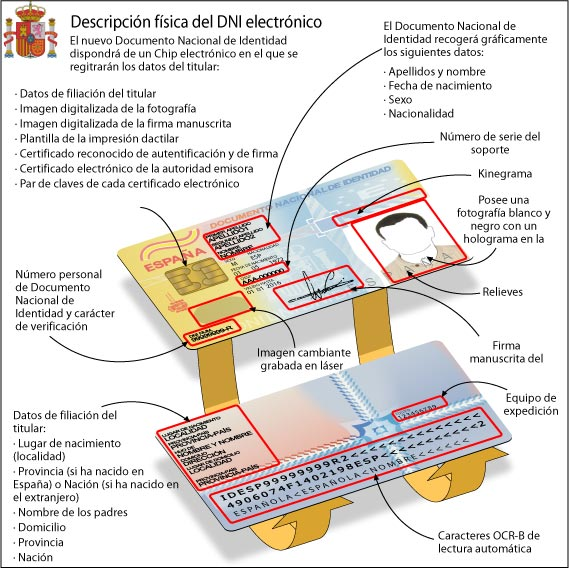
\includegraphics[scale=0.35,clip=true]{figs/dnie_descrip.jpg} 
\end{center}
\end{figure}

\end{frame}


%%%%%%%%%%%%%%%%%%%%%%%%%%%%%%%%%%%%%%%%%%%%%%%%%%%%%%%%%%%%%%%%%%%%%%%
\subsection{¿Para qué sirve el DNIe?}
\begin{frame}
\frametitle{¿Para qué sirve el DNIe?}

\begin{itemize}
\item Acreditar electrónicamente y de forma indubitada la identidad de la persona para realizar cualquier tipo de trámite.
\item \alert{Firmar} digitalmente documentos electrónicos, otorgándoles una validez jurídica equivalente a la firma manuscrita.
\item Comprobar la \alert{identidad} y la \alert{integridad} de un documento firmado.
\item Se garantiza el compromiso del titular con la firma realizada (garantía de ``no repudio'').
\item \alert{No} se contempla el uso de \alert{cifrado}. Solo firma y autenticación
\end{itemize}

\end{frame}

\subsection{Claves y certificados}
%%%%%%%%%%%%%%%%%%%%%%%%%%%%%%%%%%%%%%%%%%%%%%%%%%%%%%%%%%%%%%%%%%%%%%%

\begin{frame}
\frametitle{Conceptos a diferenciar}

\begin{itemize}
\item Claves públicas y privadas
\item Certificados
\item PIN
\end{itemize}

\end{frame}

%%%%%%%%%%%%%%%%%%%%%%%%%%%%%%%%%%%%%%%%%%%%%%%%%%%%%%%%%%%%%%%%%%%%%%%

\begin{frame}
\frametitle{Claves públicas y privadas del DNIe}

\begin{itemize}
\item La \alert{clave privada} se genera dentro del chip por un procesador que incorpora la tarjeta y nunca abandona el chip. 
\item La \alert{clave pública} se da a conocer al interlocutor en la transacción telemática. 
\end{itemize}

\end{frame}

%%%%%%%%%%%%%%%%%%%%%%%%%%%%%%%%%%%%%%%%%%%%%%%%%%%%%%%%%%%%%%%%%%%%%%%

\begin{frame}
\frametitle{Certificados del DNIe}

Con el DNI electrónico se obtienen dos certificados:

\begin{itemize}
\item El \alert{Certificado de autenticación} (\textit{Digital Signature}): para acreditar la identidad. Este certificado lleva una clave privada asociada.
	\begin{itemize}
	\item utilizado para generar mensajes de autenticación (confirmación de la identidad)
	\item acceso seguro a sistemas informáticos
	\end{itemize}
\item El \alert{Certificado de firma}: permiten firmar trámites y documentos mediante generación de ''firma electrónica reconocida''.
\end{itemize}

\end{frame}

%%%%%%%%%%%%%%%%%%%%%%%%%%%%%%%%%%%%%%%%%%%%%%%%%%%%%%%%%%%%%%%%%%%%%%%

\begin{frame}
\frametitle{Detalles de los certificados del DNIe}

\begin{itemize}
\item Los certificados del DNIe caducan (30 meses) y pueden ser revocados en cualquier momento.
\item La activación de estos certificados tiene \alert{carácter voluntario} (RD 1553/2005, de 23 de diciembre).
\item Certificado X509v3 estándar, con el bit de ContentCommitment (No Repudio) activo.
\item Utiliza para firmar SHA1.
\item Usa claves RSA de 2048 bits.
\item Un fichero CDF (Certificate Directory File) contiene los datos públicos de la tarjeta, accesibles vía comandos APDU (ISO/IEC 7816).
\end{itemize}

\end{frame}


%%%%%%%%%%%%%%%%%%%%%%%%%%%%%%%%%%%%%%%%%%%%%%%%%%%%%%%%%%%%%%%%%%%%%%%

\begin{frame}
\frametitle{El PIN del DNIe}

\begin{itemize}
\item EL PIN es la contraseña que protege la información contenida en la tarjeta (los certificados y las claves privadas y públicas) 
\item El PIN es generado aleatoriamente (``sobre ciego'') y puede ser cambiado por el usuario.
\item Permite también autorizar la función de firma. 
\item No debe confundirse el PIN con las claves (privadas o públicas) del DNIe.
\end{itemize}

\end{frame}

%%%%%%%%%%%%%%%%%%%%%%%%%%%%%%%%%%%%%%%%%%%%%%%%%%%%%%%%%%%%%%%%%%%%%%%


\begin{frame}
\frametitle{Parte hardware}

El DNI electrónico requiere el siguiente equipamiento físico:

\begin{itemize}
\item Un ordenador personal
\item Un lector de tarjetas inteligentes que cumpla el estándar ISO-7816. 
\end{itemize}

\begin{columns}

\column[t]{4cm}

\begin{figure}
	\begin{flushleft}
	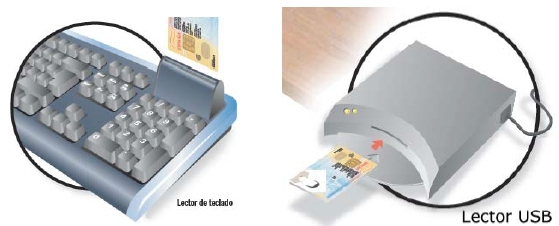
\includegraphics[scale=0.28,clip=true]{figs/lector_usb.jpg} 
	\end{flushleft}
\end{figure}

\column[t]{5cm}

Distintas implementaciones físicas de la tarjeta: 
	\begin{itemize}
	\item integradas en el teclado 
	\item externas (vía USB) 
	\item interfaz PCMCIA
	\end{itemize}

\end{columns}

\end{frame}

%%%%%%%%%%%%%%%%%%%%%%%%%%%%%%%%%%%%%%%%%%%%%%%%%%%%%%%%%%%%%%%%%%%%%%%

\begin{frame}
\frametitle{Parte software}

\begin{itemize}
\item Distintos sistemas operativos (Unix, Linux, MacOS, Windows)
\item Navegadores (Firefox, Explorer)
\item Controladores / Módulos criptográficos (CSP --Windows-- o PKCS\#11 --Unix/Linux/Mac--)
\end{itemize}

\medskip

\small
Software para Linux/Unix: \\
\url{http://www.dnielectronico.es/descargas/PKCS11_para\_Sistemas\_Unix/}

\end{frame}

%%%%%%%%%%%%%%%%%%%%%%%%%%%%%%%%%%%%%%%%%%%%%%%%%%%%%%%%%%%%%%%%%%%%%%%

\begin{frame}
\frametitle{¿Es seguro el DNIe?}

\begin{itemize}
\item Hay debate al respecto.
\item Los datos (nombre, apellidos, unidad de expedicion, nacionalidad y DNI) se pueden sacar del Certificate Directory File mediante comandos APDU.
\item Si se tiene el DNIe en el lector de tarjetas, cualquier applet puede acceder a esos datos (los datos de la parte ``pública'' de la tarjeta).
\item Infraestructura PKI: nunca se puede acceder a la clave privada.
\item Internet es un medio inhrentemente inseguro: podría estar expuesto a vulnerabilidades SSL (robo de sesión), pero como cualquier otro certificado o sesión SSL. 
\end{itemize}

\medskip

\end{frame}


%%%%%%%%%%%%%%%%%%%%%%%%%%%%%%%%%%%%%%%%%%%%%%%%%%%%%%%%%%%%%%%%%%%%%%%
\subsection{OpenDNIe}
\begin{frame}
\frametitle{OpenDNIe}

\begin{itemize}
\item Proyecto para desarrollar un módulo pkcs\#11 bajo licencia LGPL. 
\item Liderado por CENATIC (Ministerio de Industria).
\item Colaboran desarrolladores particulares y tiene el apoyo de la DGP y de la Guardia Civil.
\end{itemize}

\smallskip

\begin{center}
\url{http://forja.cenatic.es/projects/opendnie}
\end{center}

\end{frame}


%%%%%%%%%%%%%%%%%%%%%%%%%%%%%%%%%%%%%%%%%%%%%%%%%%%%%%%%%%%%%%%%%%%%%%%
\section{Certificados de la FNMT}
%%%%%%%%%%%%%%%%%%%%%%%%%%%%%%%%%%%%%%%%%%%%%%%%%%%%%%%%%%%%%%%%%%%%%%%

\subsection{FNMT-RCM}
%%%%%%%%%%%%%%%%%%%%%%%%%%%%%%%%%%%%%%%%%%%%%%%%%%%%%%%%%%%%%%%%%%%%%%%

\begin{frame}
\frametitle{Casa de la Moneda}

\begin{itemize}
\item \alert{FNMT-RCM}: Fábrica Nacional de Moneda y Timbre - Real Casa de la Moneda.
\item Entidad pública, adscrita al Ministerio de Economía y Hacienda.
\item Nace en 1893, al fusionarse la Casa de la Moneda y la Fábrica del Sello.
\item Dedicada a la fabricación de monedas, billetes, papel moneda, timbres, documentos oficiales y prestador de \alert{servicios de certificación}.
\end{itemize}

\end{frame}


\begin{frame}
\frametitle{FNMT-RCM}

\begin{itemize}
\item La FNMT-RCM, a través de su departamento \alert{CERES} (CERtificación ESpañola) ofrece certificados electrónicos para su uso (no exclusivo) ante las AA.PP.
\item El certificado FNMT es de Clase 2CA.
\item La obtención del certificado electrónico de usuario es gratuita.
\item La entidad cuenta con unos 2.5M de certificados activos vigentes (oct. 2011).
\item Tiene una validez de 3 años (2 años si es una entidad jurídica).
\end{itemize}

\end{frame}

\subsection{Certificados de FNMT}
%%%%%%%%%%%%%%%%%%%%%%%%%%%%%%%%%%%%%%%%%%%%%%%%%%%%%%%%%%%%%%%%%%%%%%%

\begin{frame}
\frametitle{Certificados de FNMT}

CERES emite los certificados de la FNMT-RCM en dos soportes:
\begin{itemize}
\item FNMT Certificado de Usuario en software
\item Certificado de usuario en Tarjeta Criptográfica
\end{itemize}

\end{frame}
 
 

%%%%%%%%%%%%%%%%%%%%%%%%%%%%%%%%%%%%%%%%%%%%%%%%%%%%%%%%%%%%%%%%%%%%%%%

\begin{frame}
\frametitle{Certificados FNMT - Software}

\begin{itemize}
\item Se usa directamente en cualquier navegador web. 
\item No precisa ningún hardware extra.
\item Pueden hacerse backups.
\end{itemize}

\end{frame}


%%%%%%%%%%%%%%%%%%%%%%%%%%%%%%%%%%%%%%%%%%%%%%%%%%%%%%%%%%%%%%%%%%%%%%%

\begin{frame}
\frametitle{Certificados en Tarjeta Criptográfica}


\begin{columns}

\column[t]{9cm}

\begin{itemize}
\item Los certificados de la FNMT se pueden almacenar y usar desde una tarjeta criptográfica.
\item Los certificados se generan en la tarjeta.
\item Más seguro que la solución software, pues no se pueden copiar y nunca salen de la tarjeta.
\item El chip dificulta técnicas de criptoanálisis, fuerza bruta o análisis diferencial.
\end{itemize}

\column[t]{3cm}
\vspace{1cm}
\begin{figure}
	\begin{flushleft}
	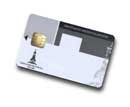
\includegraphics[scale=2.0,clip=true]{figs/criptografica.jpg} 	
	\end{flushleft}
\end{figure}


\end{columns}

\end{frame}

\subsection{Cómo funciona un certificado FNMT}
%%%%%%%%%%%%%%%%%%%%%%%%%%%%%%%%%%%%%%%%%%%%%%%%%%%%%%%%%%%%%%%%%%%%%%%

\begin{frame}
\frametitle{Cómo funciona un certificado FNMT por software}

\begin{enumerate}
\item Al solicitar un certificado de usuario, el navegador genera un par de claves. 
\item La clave privada se guarda en el navegador y la clave pública se envía a la FNMT-RCM. 
\item La FNMT-RCM asigna un código de solicitud a esa clave que es remitido vía web. 
\item Entonces hay que personarse en una oficina de acreditación con el DNI y dicho código.  
\item Finalmente, tras la acreditación, se procede a la descarga del certificado vía web. Este quedará instalado en el navegador.
\end{enumerate}

\end{frame}



%%%%%%%%%%%%%%%%%%%%%%%%%%%%%%%%%%%%%%%%%%%%%%%%%%%%%%%%%%%%%%%%%%%%%%%

\begin{frame}
\frametitle{Obtención de un certificado FNMT-RCM}

\begin{enumerate}
\item Descarga del Certificado Raíz de la FNMT-RCM (en la web de la FNMT(*))

\item (Opcional) En caso de disponer de lector de tarjetas:
	\begin{enumerate}
	\item Instalación de los drivers del lector.
	\item Instalación del software incluido junto a la tarjeta criptográfica. 
	\end{enumerate}
\item Solicitud de Certificado de Usuario (en la web de la FNMT)
\item Acreditación de la identidad (físicamente en una oficina de registro como la SS o AEAT)
\item Descarga del Certificado (en la web de la FNMT)

\end{enumerate}

\begin{center}
 (*) \url{http://www.cert.fnmt.es}
\end{center}

\end{frame}

%%%%%%%%%%%%%%%%%%%%%%%%%%%%%%%%%%%%%%%%%%%%%%%%%%%%%%%%%%%%%%%%%%%%%%%

\subsection{Ejemplo de firma digital}

\begin{frame}
\frametitle{Firma digital}

\begin{figure}
	\begin{center}
	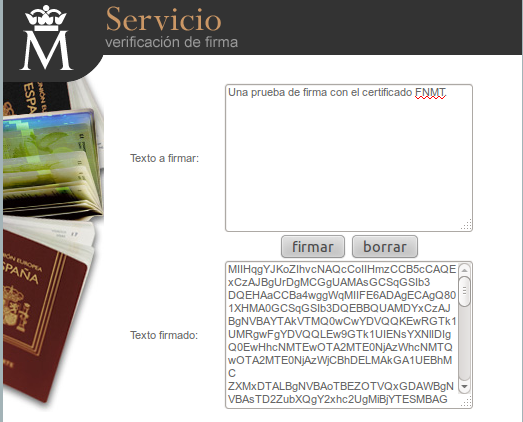
\includegraphics[scale=0.40,clip=true]{figs/firma.png} 	
	\end{center}
\end{figure}

\end{frame}


%%%%%%%%%%%%%%%%%%%%%%%%%%%%%%%%%%%%%%%%%%%%%%%%%%%%%%%%%%%%%%%%%%%%%%%

\begin{frame}
\frametitle{Verificación de firma digital}

\begin{figure}
	\begin{center}
	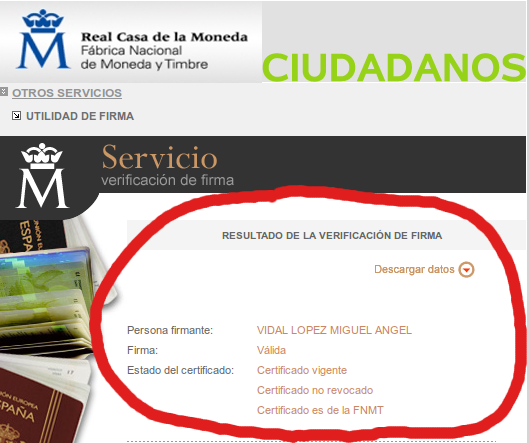
\includegraphics[scale=0.40,clip=true]{figs/firma-ver.png} 	
	\end{center}
\end{figure}

\end{frame}

%%%%%%%%%%%%%%%%%%%%%%%%%%%%%%%%%%%%%%%%%%%%%%%%%%%%%%%%%%%%%%%%%%%%%%%

\begin{frame} 
\frametitle{Referencias}

\begin{itemize}
\item Web de la FNMT (Proyecto CERES): \url{http://www.cert.fnmt.es}
\item Portal oficial del DNI electrónico (DGP): \url{http://www.dnielectronico.es}
\end{itemize}

\end{frame}



%%%%%%%%%%%%%%%%%%%%%%%%%%%%%%%%%%%%%%%%%%%%%%%%%%%%%%%%%%%%%%%%%%%%%%%

{
\frame{
\setbeamercolor{titlelike}{fg=red}
\maketitle
\begin{center}

\includegraphics[width=3cm]{format/urjc}
\hspace{1cm}

\includegraphics[width=1.8cm]{format/upm}
\end{center}
}
}

\end{document}

%%%%%%%%%%%%%%%%%%%%%%%%%%%%%%%%%%%%%%%%%%%%%%%%%%%%%%%%%%%%%%%%%%%%%%%
%%%%%%%%%%%%%%%%%%%%%%%%%%%% FIN %%%%%%%%%%%%%%%%%%%%%%%%%%%%%%%%%%%%%%
%%%%%%%%%%%%%%%%%%%%%%%%%%%%%%%%%%%%%%%%%%%%%%%%%%%%%%%%%%%%%%%%%%%%%%%


Sede Electrónica de la Admon Tributaria:
https://www.agenciatributaria.gob.es/AEAT.sede/Inicio/Inicio.shtml

Práctica:
1) Instalar y ver certificados en Firefox
2) Instalar certificado en Chrome
3) Revisar un certificado
4. Importar certificado raíz (FNMT)
5. Acceder a una página con el certificado.
6. Prueba de firma digital: http://www.cert.fnmt.es/index.php?cha=cit&sec=10&page=78&lang=es
7. Verificar firma digital: http://www.cert.fnmt.es/index.php?cha=cit&sec=10&page=77&lang=es


